\newpage
\subsection{\pVertexFitter}
\secwriter{A. Zupanc}


\paragraph{General overview}

Module performs a single kinematic fit per call. For example, in the following decay chain of $B$ mesons,
\begin{eqnarray*}
 B^- & \to & D^0 \pi^-\\ 
& & \hookrightarrow K^-\pi^+,
\end{eqnarray*}
two decay vertices exist -- $B$ and $D$ meson decay vertices. Using the \pVertexFitter module both
decay vertices can be reconstructed one after another by performing the following two steps:
\begin{itemize}
 \item 1. step: $D^0 \to K^- \pi^+$ decay vertex reconstruction,
 \item 2. step: $B^- \to D^0 \pi^-$ decay vertex reconstruction (results from step 1 are used and needed).
\end{itemize}

Module {\tt DecayChainVertexFitter} described in section~\ref{sec:modules:decayChainVertexFitter} can fit the entire decay 
chain (both decay vertices) given above in one single step.

\subsubsection{Input and control parameters}

Parameters of the \pVertexFitter module are:
\begin{itemize}
 \item {\bluett pListName} (string): name of the input \pList 
 \item {\bluett decayString} (string): specifies which daughter particles are included in the kinematic fit (see 
 section \ref{sec:tools:decayDescriptor} for a description of the \decayString)
 \begin{itemize}
  \item default value: {\color{red}\tt \bf empty string} $\rightarrow$ all daughter particles are included in the fit
  \item example 1: {\color{red}\tt D0 -> \string^K- \string^pi+}
  \begin{itemize}
   \item all daughters are included 
   \item same as default
  \end{itemize}
  \item example 2: {\color{red}\tt D0 -> \string^pi- \string^pi+ K\_S0}
  \begin{itemize}
   \item $D^0$ decay vertex is determined using $\pi^+$ and $\pi^-$ tracks only; neutral kaon is not included into the fit;
  \end{itemize}
  \item example 3: {\color{red}\tt  D\_s+ -> (phi -> \string^K+ \string^K-) \string^pi+}
  \begin{itemize}
   \item $D_s^+$ decay vertex is determined by fitting $K^+$, $K^-$ and $\pi^+$ tracks to a common point
   \item $\phi$ is strongly decaying resonance with very short lifetime and it makes no sense to fit its decay vertex separately
  \end{itemize}
  \item example 4: {\color{red}\tt  B0 -> (D*+ -> \string^D0 pi+) (D*- -> \string^anti-D0 pi-)}
  \begin{itemize}
   \item $B^0$ decay vertex is determined by fitting $D^0$ and $\overline{D}{}^0$ from $D^{\ast}$ decays to a common point; slow pions 
         are not included;
  \end{itemize}
 \end{itemize}
 \item {\bluett fitType} (string): type of the kinematic fit (see \cite{fitters} for details)
 \begin{itemize}
  \item {\redtt vertex}: this is default value
  \item {\redtt mass}: mass constrained fit (no vertex is determined in the fit)
  \item {\redtt massvertex}: mass-constrained-vertex fit
 \end{itemize}
 \item {\bluett withConstraint} (string): whether an additional constraint on vertex should be imposed
 \begin{itemize}
  \item default value: {\color{red}\tt \bf empty string} $\rightarrow$ no additional constraint
  \item {\redtt ipprofile}: the vertex is constrained to lie within {\tt IPProfile}
  \item {\redtt iptube}: the vertex is constrained to lie within {\tt IPTube}
  \item {\it How could a decay/production vertex of some particle within the decay chain be specified here? Need to discuss it with C. Oswald 
  if \decayString can be used here.}
 \end{itemize}
 \item {\bluett updateDaughters} (bool): whether the momenta of daughter particles should be updated
 \begin{itemize}
  \item default value: {\color{red}\tt \bf false} $\rightarrow$ only mother momentum is updated
  \item {\color{red}\tt \bf true}: mother and daughter momenta are updated (see below for implications/consequences)
 \end{itemize}  
\end{itemize}

\subsubsection{Action description}

Module loops over all mother particles within the specified \pList (via {\tt pListName} module parameter) and performs on each of them specified
kinematic fit as instructed by the user via {\tt decayString, fitType} and {\tt withConstraint} parameters. By default as a result of this
action ({\tt updateDaughters=false}) the following data members of the mother particle are updated with the results of the kinematic fit:
\begin{itemize}
 \item 4-momentum,
 \item position/decay vertex,
 \item $7\times7$ error matrix,
 \item $\chi^2$ value,
 \item number of degrees of freedom.
\end{itemize}
The data members of daughter \particle objects are not changed in any way. By default the module has no impact 
on the \storearray{{\tt Particle}} or \storeobjptr{ParticleList} as illustrated in the figure below (The green font color  for $D^0$ \particle objects with indices 8 and 9
in the {\it after} figure just indicate that the mother \particle objects were modified by the action.).

\newpage
\begin{center}
 {\color{red} Default action ({\tt updateDaughters=false}):}\\
{\color{darkgreen} only mother particle is updated}\\
\vspace{0.2cm} 
{\bf\large Before}\\
\vspace{0.2cm}
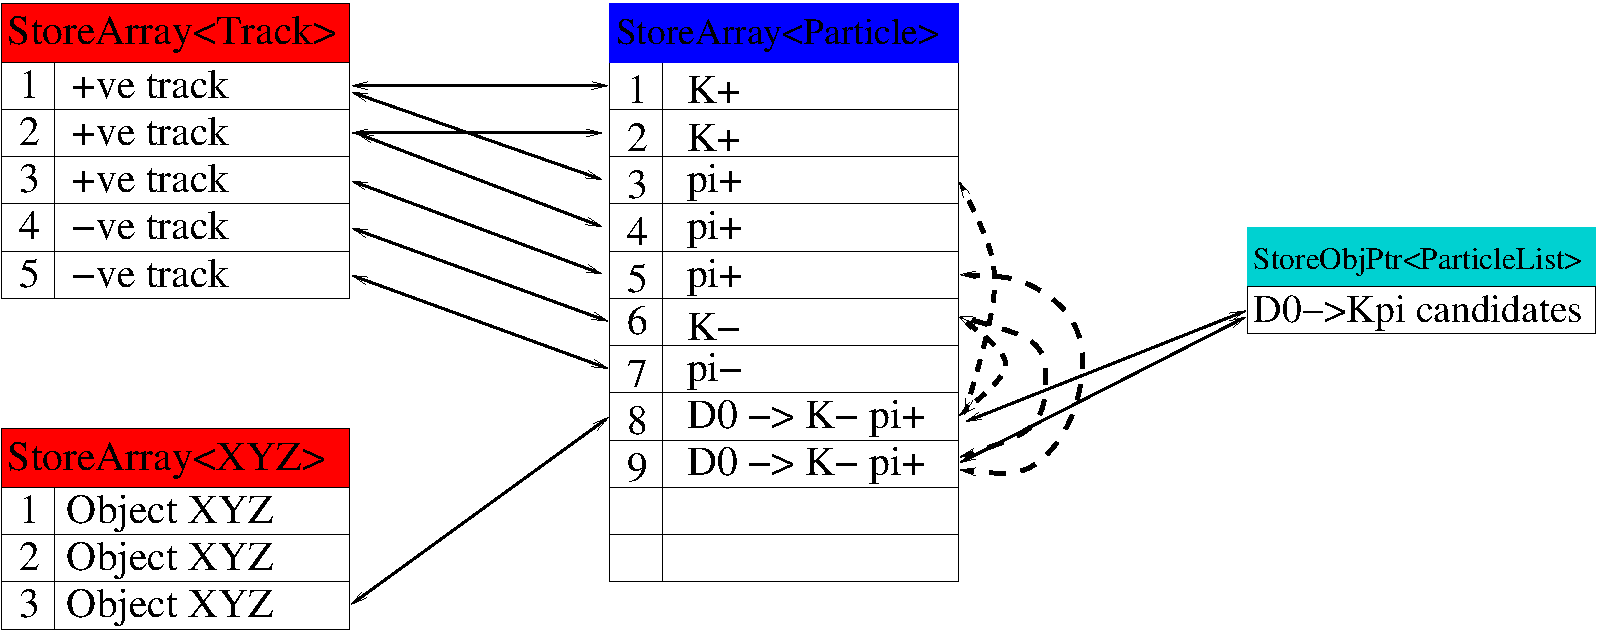
\includegraphics[width=0.9\textwidth]{AnalysisModules/figs/vertexingDataStore.pdf}\\
\vspace{0.2cm}
{\bf\large After}\\
\vspace{0.2cm}
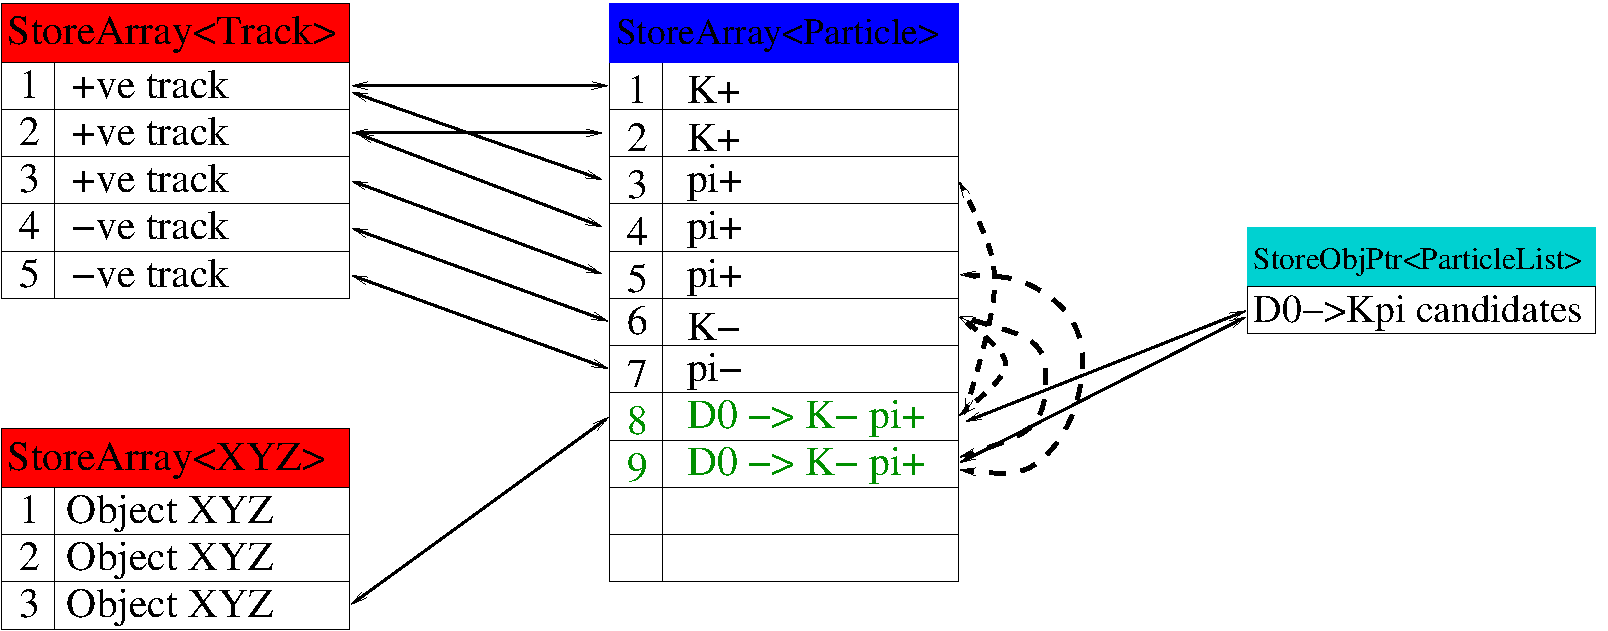
\includegraphics[width=0.9\textwidth]{AnalysisModules/figs/vertexingDataStoreB.pdf}
\end{center}

Since in the above case $D^0$ candidates (\particle objects under index 8 and 9) share the same daughter particle (the $K^-$) it is clear
that if we wish to update the daughter momenta we need to make a copies of daughter \particle objects that will be unique to each $D^0$
candidate. Therefore, if it is necessary in the physics analysis to know the fitted momenta of daughter particles (note that this is
in most analyses not the case), user has to turn on the {\tt updateDaughters} flag (set it to {\tt true}). As a consequence the entire 
decay chain (mother and daughter \particle objects) is copied within the \storearray{{\tt Particle}} and the corresponding indices in the
\storeobjptr{ParticleList} are updated as illustrated in the figure below. In addition, all \basf\ \relation{s} are copied.

\newpage
\begin{center}
 {\color{red} Optional action ({\tt updateDaughters=true}):}\\
{\color{darkgreen} mother and daughter particle objects are copied and their momenta are updated}\\
\vspace{0.2cm} 
{\bf\large Before}\\
\vspace{0.2cm}
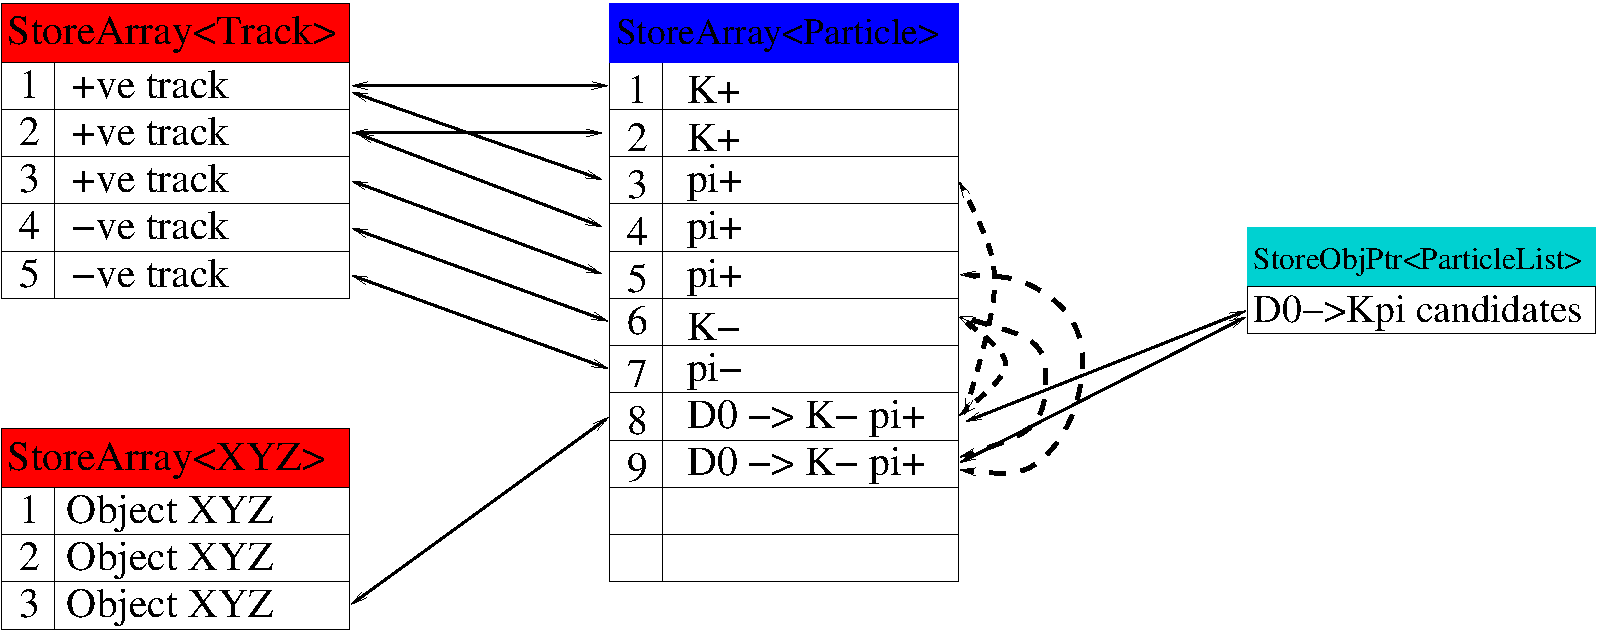
\includegraphics[width=0.9\textwidth]{AnalysisModules/figs/vertexingDataStore.pdf}\\
\vspace{0.2cm}
{\bf\large After}\\
\vspace{0.2cm}
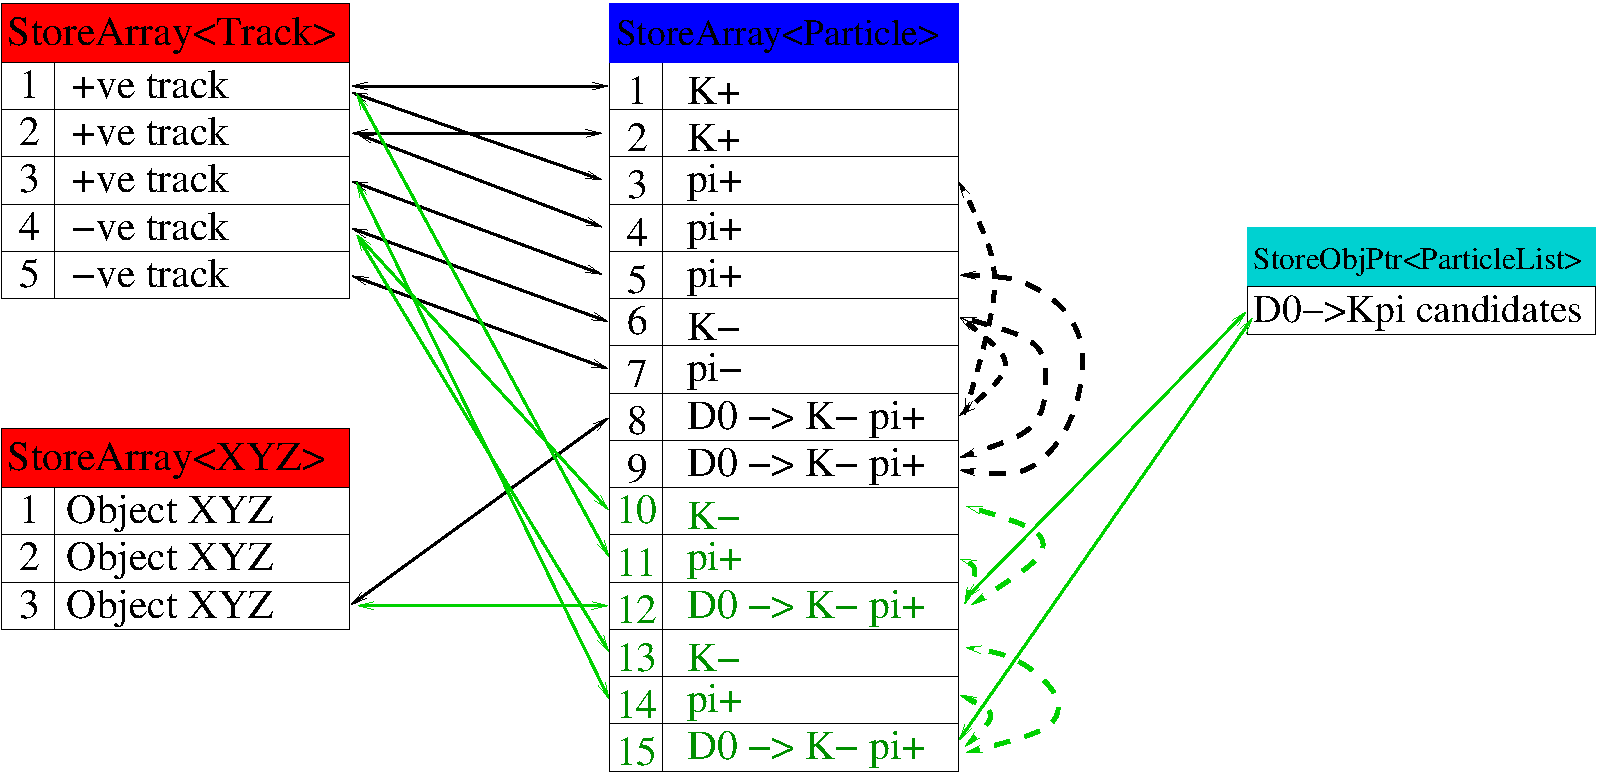
\includegraphics[width=0.9\textwidth]{AnalysisModules/figs/vertexingDataStoreC.pdf}
\end{center}
